%\begin{wrapfigure}{r}{0.9\textwidth}
%	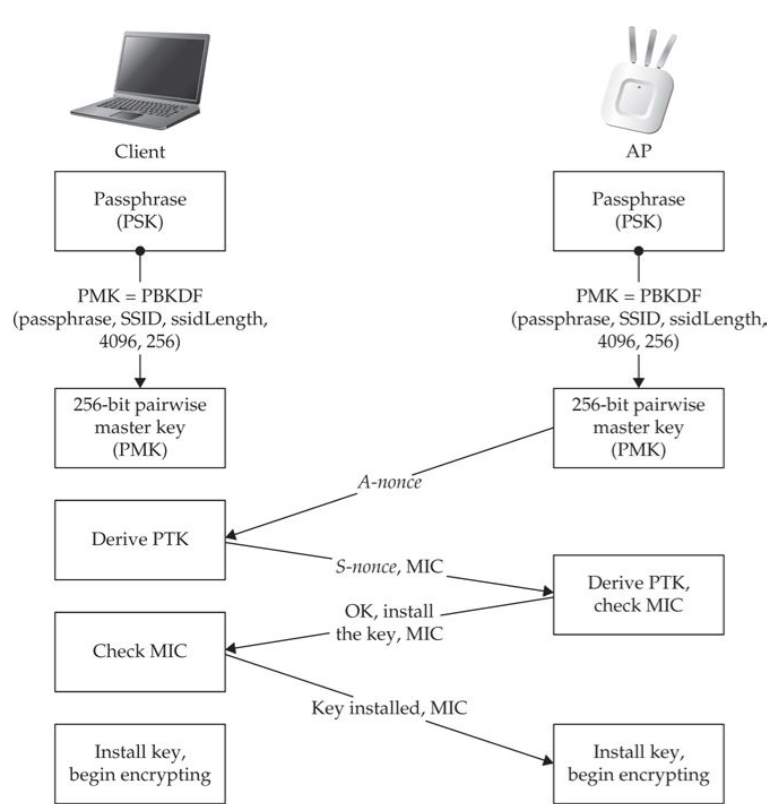
\includegraphics[width=1.0\linewidth]{images/wpa/four-way-handshake.png}
%	\caption[WPA: The four-way handshake]{WPA: \textit{The four-way handshake} (Quelle: \fullcite[][151]{WrightCache201503})}
%\end{wrapfigure}

\chapter{Allgemein}
\label{ch:general}
Dieses einleitende \chapref{ch:general} gibt einen groben Überblick zum Thema Wireless. Es wird auf Modis, Paket Typen, Paket Adressen, Verschlüsselungstechniken (allgemein) und Angriffe eingegangen.

\section{Modis}
Eine drahtlose Kommunikation kann in drei verschiedenen Modis betrieben werden.
Meist funktioniert die Kommunikation via einen \gls{apLabel}, über den alles läuft. Der \gls{apLabel} leitet die Pakete weitere und kontrolliert die Verbindungen.
Nebst der \gls{apLabel}-Variante gibt es noch den ad-hoc oder \gls{ibssLabel} Modus. Auch hier gibt es einen \gls{apLabel}, aber die Pakete müssen nicht zwingend über jenen geleitet werden, sondern die Stationen können direkt miteinander kommunizieren.\footcite[][38]{WrightCache201503}

Nebst den zwei grundlegenden Modis existiert der \textit{Wi-Fi Direct} Modus, der eine direkte Verbindung zweier Geräte ohne \gls{apLabel} erlaubt.\footcite{WiFi_Direct_Wikipedia_the_free_encyclopedia_2015-04-17}

\section{Paket Typ}
Die Pakete können in drei Kategorien eingeteilt werden:
\begin{itemize}
	\item Data (Daten): Mit \textit{Data}-Paketen werden alle Informationen bezeichnet, die grundsätzlich übertragen werden müssen.
	\item Management (Verwaltung): \textit{Management} Pakete sind alle Pakete, welche Informationen zum Netzwerk bereitstellen (z.B. \glspl{glos:beaconLabel} und Deauthentication Pakete)
	\item Control (Kontrolle): \textit{Control}-Pakete steuern die Kommunikation. Sie regeln z.B. wer wann senden darf (z.B.: \gls{rtsLabel} und \gls{ctsLabel}).
\end{itemize}

\section{Adresse}
Jedes Paket beinhaltet, nebst Quell- und Zieladresse, auch eine \gls{bssidLabel}, welche den \gls{apLabel} identifiziert (meist entspricht sie der \gls{macLabel}-Adresse des \gls{apLabel}).


\section{Verschlüsselungstechnik}
Es gibt zwei Arten auf welche die Kommunikation verschlüsselt werden kann: \gls{wepLabel} (\chapref{ch:wep}) und \gls{wpaLabel} (\chapref{ch:wpa}).
Beide Arten unterstützen die \gls{pskLabel} (vorzeitig ausgetauschte Schlüssel) Methode, bei der für alle Nutzer der gleiche Schlüssel für Authentifizierung und Verschlüsselung verwendet wird.

\section{Angriffe}

\subsection{Sicheheitslevel}
Netzwerke können grob in drei Sicherheitslevel eingestuft werden:\footcite[][115]{WrightCache201503}
\begin{itemize}
	\item \textbf{Geringe Sicherheit:} Von geringer Sicherheit spricht man, wenn man ohne oder mit sehr geringen Aufwand Sicherheitsmassnahmen umgehen kann.
	\item \textbf{Mittlere Sicherheit:} Mittlerer Sicherheit, kann mit mässigem Einsatz von Ressourcen (Zeit und Wissen) umgangen werden (z.B. ein \gls{wepLabel}-Schlüssel oder ein schwacher \gls{wpaLabel}-Schlüssel).
	\item \textbf{Hohe Sicherheit:} Hohe Sicherheitsmassnahmen können kaum oder nur mit extremen Aufwand umgangen werden.
\end{itemize}

\subsection{Angriffsarten}
Es grundsätzlich zwei Angriffsarten: \textit{aktiv} und \textit{passiv}.
\begin{itemize}
	\item \textbf{aktiv:}
	Bei der aktiven Angriffsart werden mit Hilfe verfügbaren Informationen (z.B. von \glspl{glos:beaconLabel}) verschiedene "`Erforschungs"' (probe) Requests verschickt.
	Es wird auf Antworten die weitere wichtige Informationen verraten gehofft.
	Der generelle Datenverkehr kann mit aktiv Tools nicht abgehört werden.

	\item \textbf{passiv:}
	Passiv Angriffe sind mächtiger. Dazu wird die Netzwerkkarte in den \gls{glos:monitorModeLabel} umgeschaltet.
	So können alle Pakete eines Channels, unabhängig der \gls{ssidLabel}'s (sprich über mehrere Netzwerke), abgefangen werden.

\end{itemize}

\subsection{Angriffsziele}
Ziel eines Angriffes kann das Abhören (evt. inkl. Manipulation) oder der vollständigen Netzwerkzugriff (via \gls{pskLabel}) sein.
Meist wird der vollständige Netzwerkzugriff angestrebt, da dann auch alle Kommunikation abgehört werden kann.

\section{Test Umgebung (Soft- und Hardware)}
\label{sec:testEnvroiment}
\subsection{System}
Für die praktischen Beispiele wurde ein Apple \textit{Mac Book Air (early 2014)} mit einem 1.4GHz Intel Core i5 Prozessor und 8 GB RAM verwendet. Als Grafikkarte wurde die eingebaute, standard \textit{Intel HD Graphics 5000} mit 1536 MB Shared Memory verwendet.
Als Betriebssystem ist OS X \textit{Yosemite} Version 10.10.2/3  installiert.

Die eingebaute Netzwerkkarte \textit{AirPort Extreme} mit der Firmware \textit{Broadcom BCM43xx 1.0 (7.15.159.13.12)} unterstützt das Aufzeichnen aller \gls{wlanLabel}-Daten im \textit{monitor mode} (\textit{sniffing}), jedoch kein Senden von manipulierten Paketen (\textit{packet-injection}).
%Als Netzwerkkarte wurde die eingebaute \textit{AirPort Extreme} mit der Firmware \textit{Broadcom BCM43xx 1.0 (7.15.159.13.12)} verwendet.

Falls nichts anderes erwähnt wird, wurde immer soeben beschriebenes System verwendet.


\subsection{Software}
\textit{Mac OS X} stellt, innerhalb von Xcode\footcite{Xcode_Apple_Developer_2015-04-06}, bereits nützliche Wireless Analyse Tools unter dem Namen \textit{Wireless Diagnostics} zur Verfügung.

\begin{framed}
	\textbf{Bemerkung:} Obwohl das \textit{KisMac2}\footcite{IGR_Software_KisMac2_2015-04-06} viel erwähnt wird, hat sich dieses Programm während dieser Arbeit nicht bewährt. Es stürzte vermehrt ab. Darum die Empfehlung mit dem von \textit{Wireless Diagnostics} bereitgestellten \textit{airport} Konsolen-Programm zu arbeiten.
\end{framed}

Zudem kann via \textit{Homebrew}\footcite{Homebrew__The_missing_package_manager_for_OS_X_2015-04-06} die \textit{Aircrack-ng 1.1}\footcite{Aircrack-ng_2015-04-06} Programm Sammlung installiert werden.
\textit{\textit{Aircrack-ng}} unterstützt \textit{Mac OS X} zwar nicht vollständig, es können aber folgende Pakete genutzt werden: \textbf{\textit{aircrack-ng}}, \textit{packetforge-ng}, \textit{ivstools} and \textit{makeiv}.

Anstelle von \textit{airodump-ng}, wird das OS X Konsolen-Programm \textit{airport} verwendet.
